\documentclass[conference]{IEEEtran}
\IEEEoverridecommandlockouts
% The preceding line is only needed to identify funding in the first footnote. If that is unneeded, please comment it out.
\usepackage{cite}
\usepackage{amsmath,amssymb,amsfonts}
\usepackage{graphicx}
\usepackage{textcomp}
\usepackage{xcolor}
\def\BibTeX{{\rm B\kern-.05em{\sc i\kern-.025em b}\kern-.08em
    T\kern-.1667em\lower.7ex\hbox{E}\kern-.125emX}}
\title{
\vspace{1cm}
{
\includegraphics[width=0.15\textwidth]{/storage/emulated/0/FWC1/esp/IMG-20241021-WA0004.jpg} \\ ESP32 Assignment} }
\author{Sivva Pranaykumar \\ Roll No: FWC22273\\ sivvapranay.s@gmail.com}
 \begin{document}
\maketitle
 \section {ABSTRACT}
This project demonstrates the implementation of a 2x1 multiplexer (MUX) using an Arduino, where one input is passed through an inverter before reaching the MUX. The selection line determines whether the inverted or non-inverted input is routed to the output. The final output is indicated by an LED, which blinks if the output is HIGH (1) and remains OFF if the output is LOW (0). This project integrates basic digital logic with physical output representation using an LED, suitable for educational purposes in understanding multiplexers and simple digital systems.
 
 \begin{figure}[h]
 \centering
 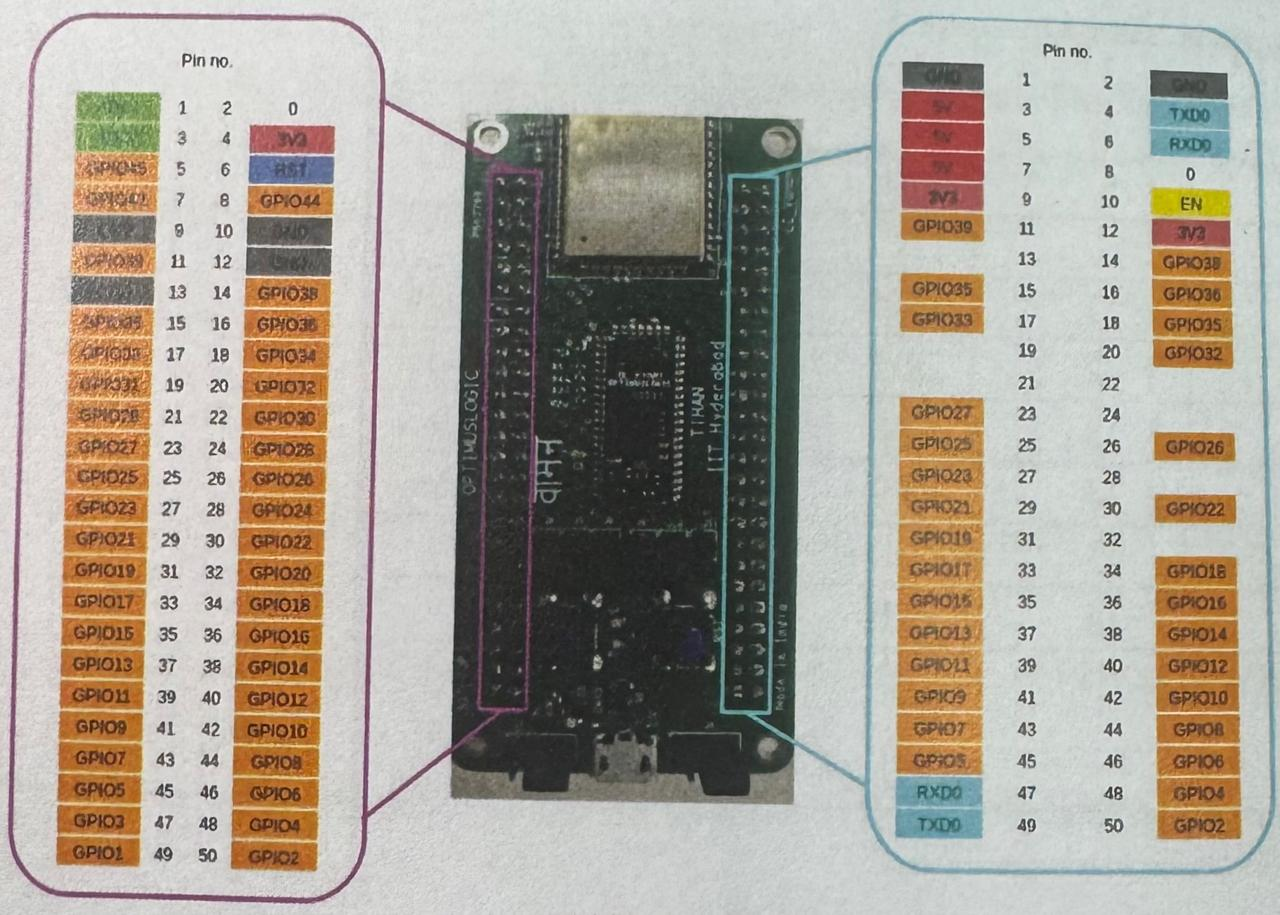
\includegraphics[width=0.35\textwidth]{/storage/emulated/0/FWC1/esp/IMG-20241024-WA0005.jpg}
 \caption{\label{fig:Gates} Vaman pinout Right side ESP32}
 \end{figure}
 
\section{COMPONENTS}
The required components list is given in Table I.

 \begin{table} [htbp]
\centering
\begin{tabular}{| c | c | c |} \hline
Components & Value & Quantity \\\hline
LEDs &  & 1 \\ \hline
Vaman &  & 1 \\ \hline
Jumper Wires &  & 10 \\ \hline
Breadboard & & 1 \\ 
\hline
\end{tabular}
\vspace{0.1cm}
\caption{\label{tab:components} List of required components.}
\end{table}

\section{PROCEDURE}
Make the connections between Vaman and LED as per Table II.

Connect Input 0 to Arduino pin 2.  
Connect Input 1 to Arduino pin 3.  
Connect the selection line (S) to Arduino pin 4.  
Connect an LED to Arduino pin 5 (through a 330\(\Omega\) resistor for current limitation).  
Apply different combinations of inputs (Input 0, Input 1, and Selection line S).  
Observe the behavior of the LED to confirm correct MUX operation.  
Ensure that the common ground is connected for all components.  
Record the LED states (blinking or OFF) based on different input conditions and selection line values.

 \begin{table}[htbp]                                       
\centering                                                          
\begin{tabular}{| c | c | c |} \hline                                
\textbf{Arduino Pin} & \textbf{Signal Connection} & \textbf{Description} \\\hline 
Pin 2 & input 0 & input 0 to be inverted \\ \hline                     
Pin 3 & input 1 & Direct input 1\\ \hline                                 
Pin 4 & Selection line (S) & Controls which input is selected \\ \hline    
Pin 5 & LED & Output (LED to blink or stay OFF) \\ \hline                                                                                  
\end{tabular}                                                        
\vspace{0.1cm}                                                       
\caption{\label{tab:connections} Pin connections for the MUX circuit.}                                       
\end{table}

\section{RESULTS}
After implementing the code and wiring the components:  
- When S = 0, the output of the MUX reflects the inverted Input 0. The LED blinks if the inverted input is HIGH and remains OFF if it is LOW.  
- When S = 1, the output of the MUX reflects Input 1. The LED blinks if Input 1 is HIGH and remains OFF if it is LOW.  

The truth table matches the expected logic for a 2x1 MUX with one inverted input.  
https://github.com/Pranaykuma/FWC-1/blob/main/ESP32/main.cpp 
 \begin{table}[htbp]                                       
\centering                                                          
\begin{tabular}{| c | c | c | c | c | c |} \hline                                
\textbf{Input 0} & \textbf{Input 1} & \textbf{S} & \textbf{Inverted Input 0} & \textbf{Output (Y)} & \textbf{LED State}\\\hline 
0 & 0 & 0 & 1 & 1 & Blinking (ON) \\ \hline                     
0 & 0 & 1 & 1 & 0 & OFF  \\ \hline                                 
1 & 0 & 0 & 0 & 0 & OFF  \\ \hline    
1 & 1 & 1 & 0 & 1 & Blinking (ON)  \\ \hline                                                                           
\end{tabular}                                                        
\vspace{0.1cm}                                                       
\caption{\label{tab:truth} Truth table for the MUX circuit.}                                       
\end{table}

\begin{figure}[h] 
	\centering 
	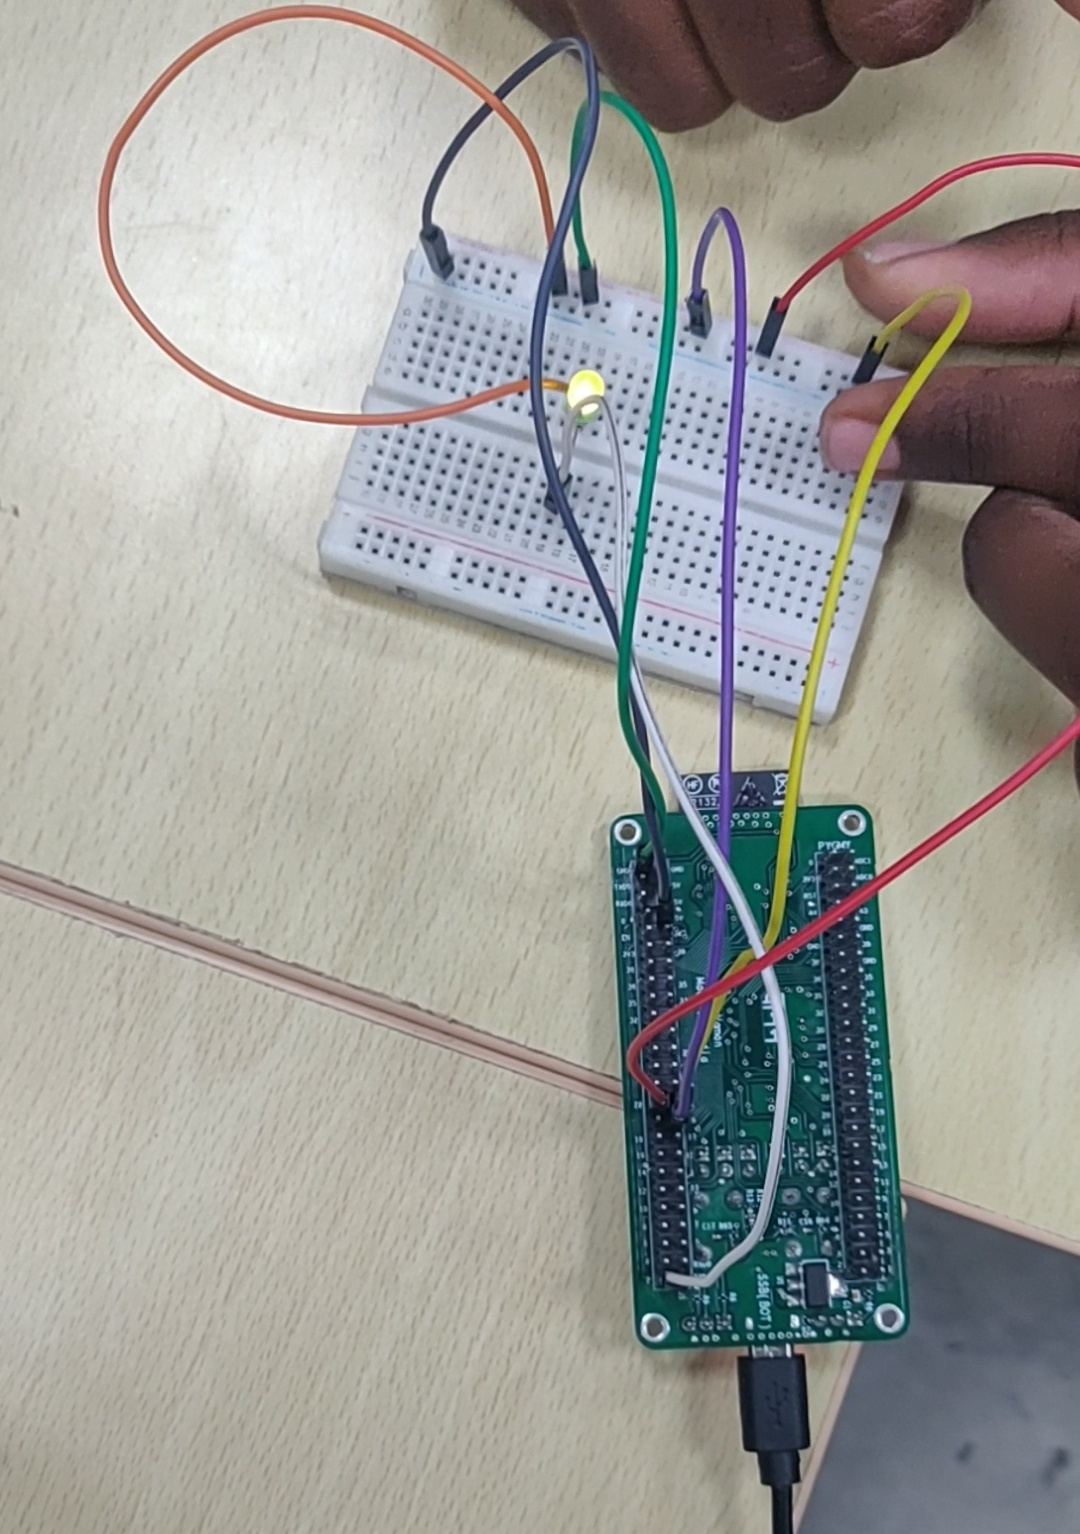
\includegraphics[width=0.4\textwidth]{/storage/emulated/0/Download/Screenshot_20241024-115945__01.jpg}
	\caption{\label{fig:output} Final output LED state based on MUX operation.}    
\end{figure}

\section{CONCLUSION}
This project successfully demonstrates the functionality of a 2x1 multiplexer with an inverter on one input, implemented using an Arduino. The MUX output is accurately reflected by an LED, which blinks for a HIGH (1) output and remains OFF for a LOW (0) output. The observed behavior of the LED corresponds to the expected truth table of the MUX, verifying the correct operation of the digital logic system. This simple project helps to illustrate the concepts of multiplexers, inversion, and selection logic, providing an effective teaching tool for digital systems and microcontroller interfacing.

\end{document}

